% 本章研究聚焦于用水者决策过程与环境之间的反馈过程进行建模。
% 使用多主体模型黄河农业灌溉主体对流域水资源分配制度的决策过程,并从“主体规则的设计”、“模块构建与耦合”、“数据输入与分析”三个方面介绍本章的研究方法。

\subsection{主体规则的设计}

本小节将分别从个体尺度、地区尺度、流域尺度介绍多主体模型的规则设计,三者的关系如图\ref{ch6:fig:framework}所示:
(1)个体尺度的灌溉主体是进行农业生产的基本单位,基于环境信息和制度条件做出具体用水决策;
(2)地区是灌溉主体受分水制度影响的主要尺度,流域系统的水资源额度分配体现在主体交互中;
(3)流域尺度则给丁了模型的环境背景,例如主体分布、水文气候条件、主体交互网络。
% 模型的主要目的是分析流域水资源分配制度如何影响农业灌溉主体的用水来源:用多少地下水?
% 将小麦、玉米、水稻三种主要粮食作物种植用水来源在月尺度区分为自然降水、地表水、地下水,并分析了地表分水制度变化对地下水开采量的影响。

\begin{figure}[htb]
    \centering
    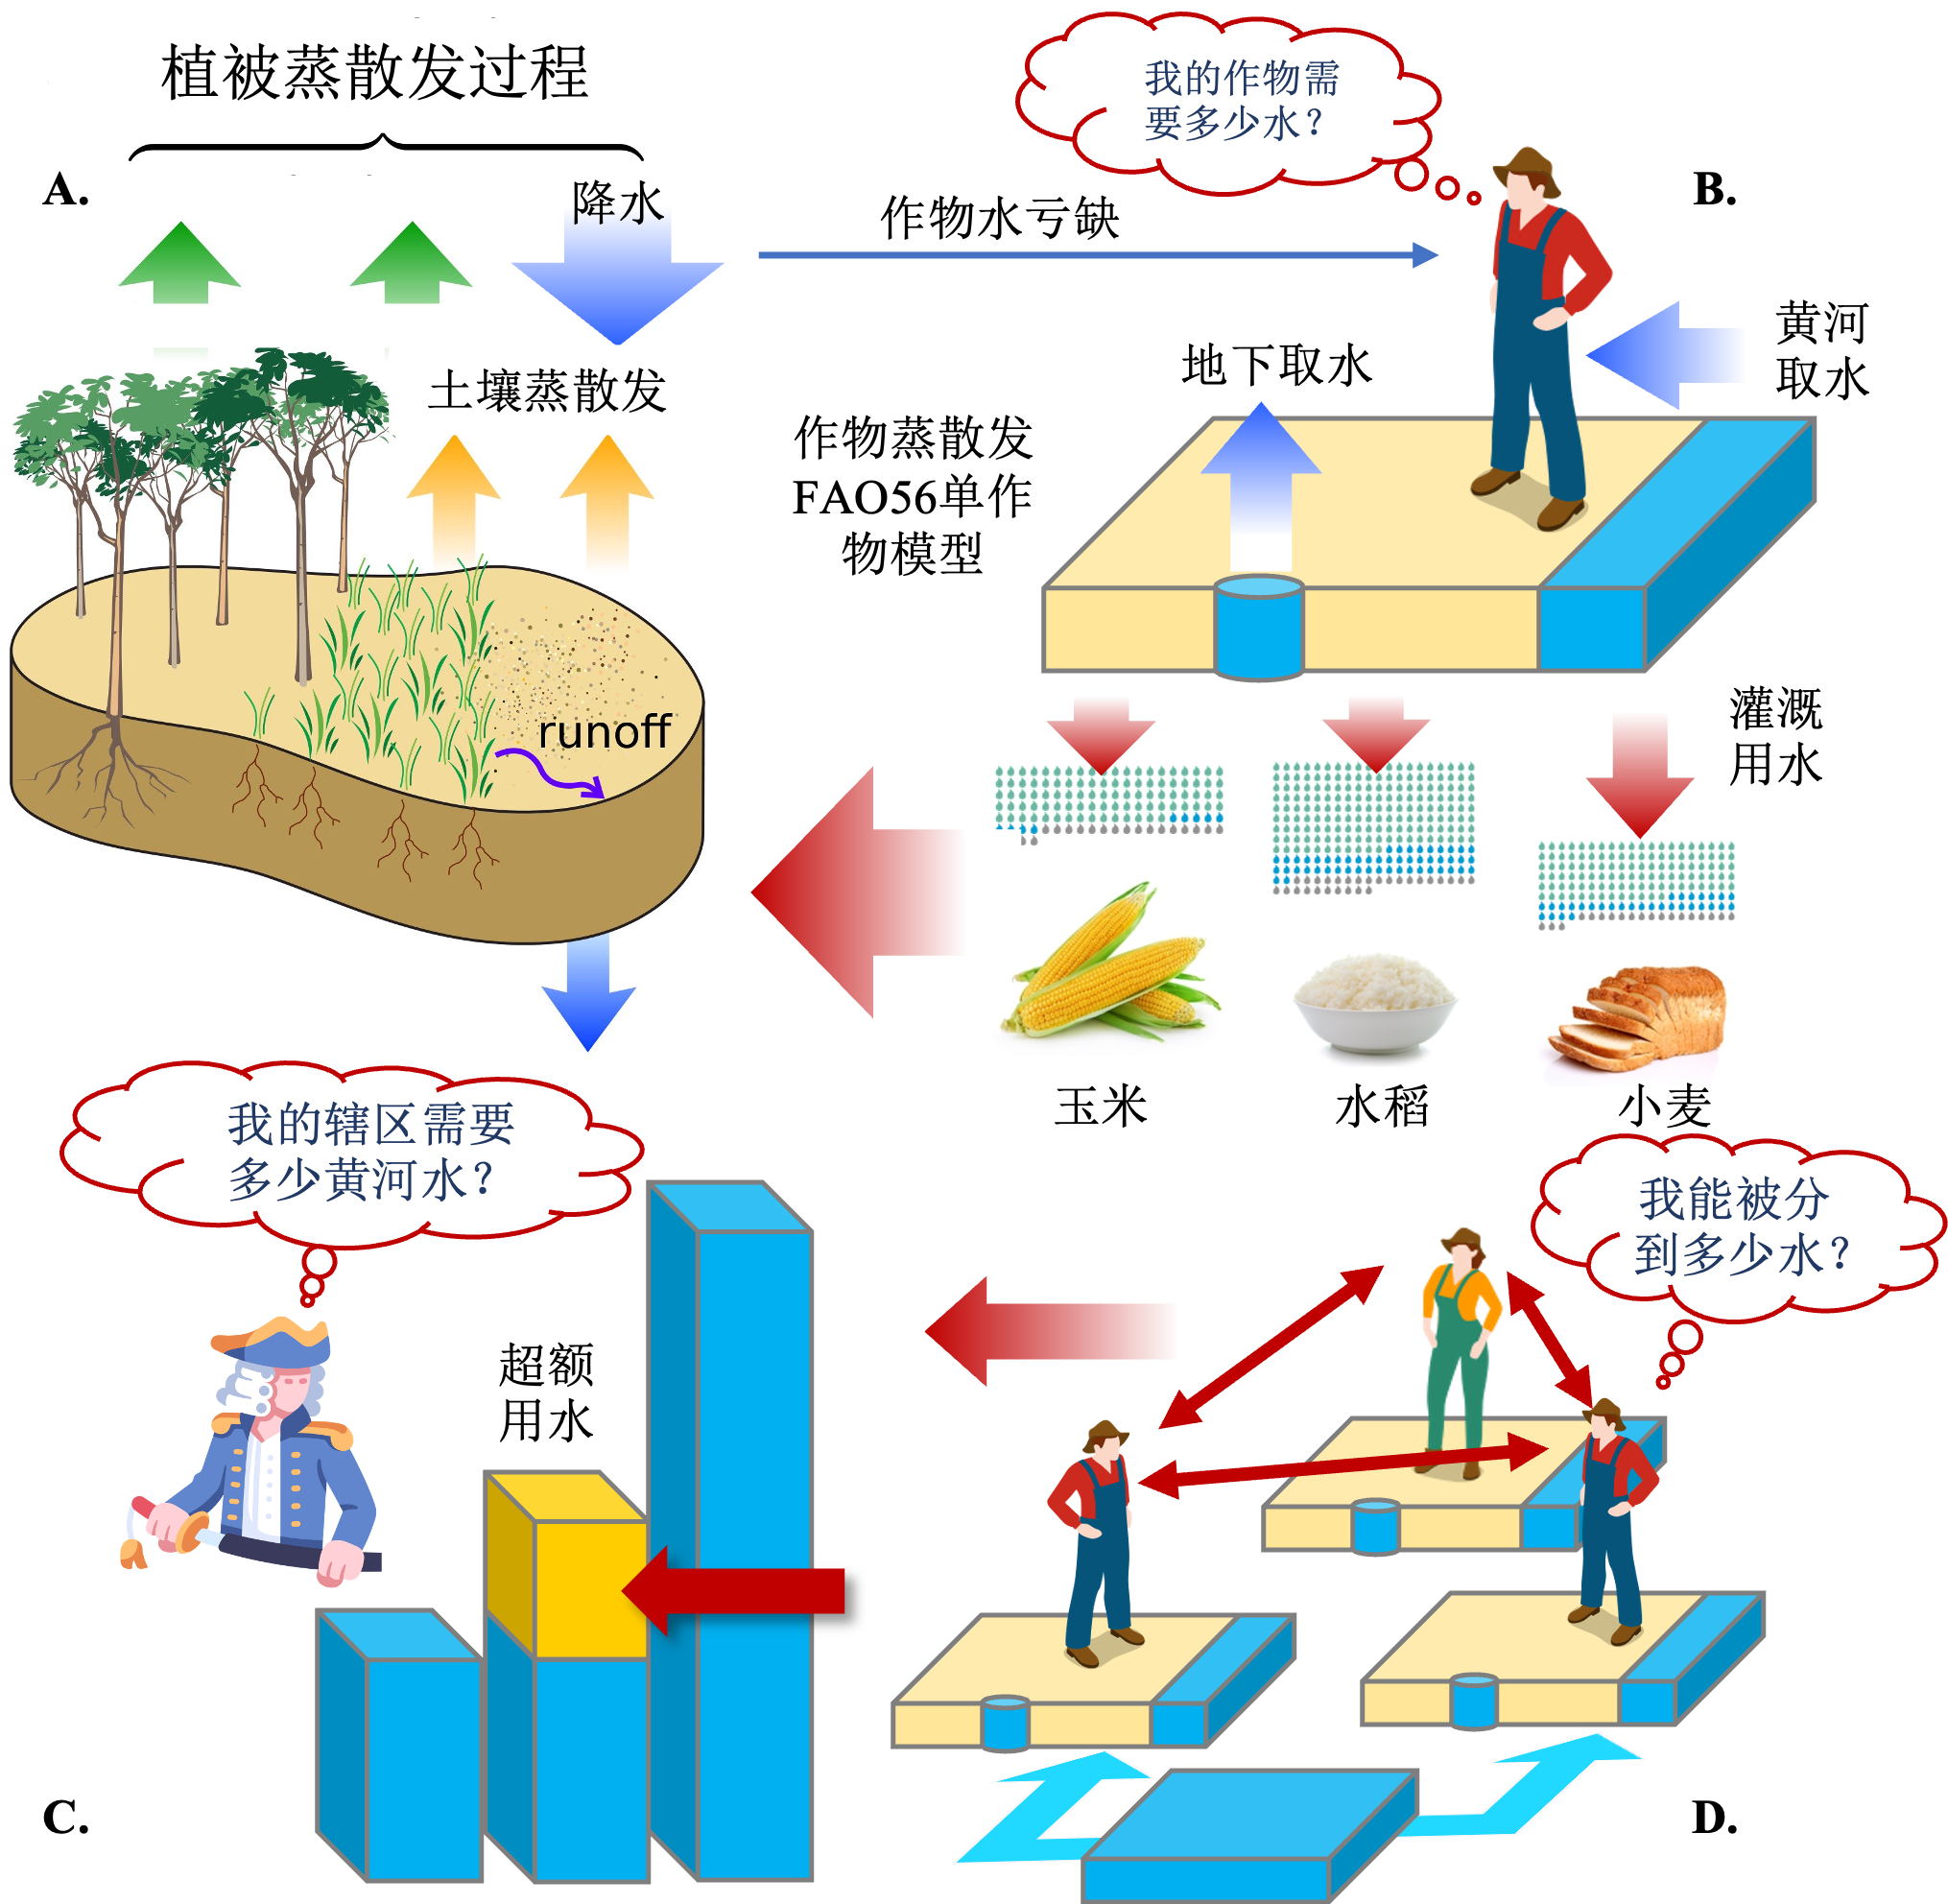
\includegraphics[width=0.8\textwidth]{img/ch6/ch6_framework.png}
    \caption[多主体模型的设计框架]{多主体模型的设计框架。
        \textbf{A.} 自然模块:水文气候条件、流域主体的作物选择和灌溉策略如何影响作物蒸散发。
        \textbf{B.} 人类模块(个体尺度):流域内的灌溉主体在给定水文气候条件、给定配额上限/下限的情况下如何决定其用水来源及用水量;
        \textbf{C.} 地区尺度:体现制度变化对区域总可用水配额的影响。
        \textbf{D.} 流域尺度:体现流域系统的主体分布、主体网络结构特征对主体博弈决策的影响。
    }\label{ch6:fig:framework}
\end{figure}

\subsubsection{个体尺度:用水决策}

对单个农民主体来说,决策核心是对天然降水之外的作物水亏缺进行人为灌溉补给。
对某个位于$x, y$的农民主体$f$而言,其支持作物生长的总用水$W_f$包括天然降水$W_{prec, x, y}$和取用水$WU_f$两部分,符合式\ref{ch6:eq:w}所示的水平衡:

\begin{equation}
    \label{ch6:eq:w}
    W_f = W_{p} + WU_{f} = \min{prec_{x, y}, ETc_{x, y}} + WU_{f}
\end{equation}

其中$W_{p}$是作物生长利用的天然降水量,等于作物蒸散发和降水量的较小值,根据主体所处的坐标位置($x, y$)直接从自然模块调用相应属性,作物蒸散发$ETc_{x, y}$则采用国际粮农组织(FAO)推荐的单作物系数法,由潜在蒸散发和作物蒸散发系数$Kc_{x, y}$计算得到(见式\ref{ch6:eq:etc})。

若降水量大于作物蒸发量,则说明自然降水已经满足作物生长,不再需要额外取水,即$WU_{f} = 0$。对于大多数需要取水灌溉的区域,作物蒸发量$ETc_{x, y} > prec_{x, y}$,可将水亏缺$W_{deficits}$定义为考虑灌溉损失后的作物蒸散发与实际降水量之间的差,且由于在灌溉中不可避免产生水量损失,参考已有研究使用系数$k_{loss}$对其进行修正\cite{chen2023}:

\begin{equation}
    \label{ch6:eq:deficits}
    W_{deficits} = \frac{ETc_{x, y} - prec_{x, y}}{k_{loss}}
\end{equation}

生产实际中不可能做到完全按照作物的水亏缺决定灌溉取水量,实际灌溉水量受到农民经验与节水灌溉设施等多因素影响,因此作物水亏缺$W_{deficits}$和实际灌溉取用水量$WU$之间仍存在较大差异,而二者比例$\frac{W_{deficits}}{WU}$可作为灌溉效率的指示。
本章研究中,对于每个地级市来说实际总取水量$WU$是外生变量,可以直接从外部数据中获取,根据用水量的年际统计数据将尺度下降到月尺度,可得每个地级市在作物生长季在第$i$($i \in [1, 12]$)月的实际取水量。

本模型在每步模拟中,可将位于$x, y$的灌溉主体$f$的作物生长用水来源$WU_f$进一步分为地表水来源$W_s$和地下水来源$W_g$两部分($WU = W_g + W_s$),具体用水决策及模型计算顺序如下:
(1)若$W_{deficits} \leq 0$,说明降水已经满足了需求,则作物生长水源$W$就完全由降水提供,即$W = W_p = prec_{x, y}$, $WU_f = W_{s} = W_{g} =0$;
(2)否则,对于需求$WU_f > 0$,假定农民$f$首先考虑从地表水获得,根据自己的地表水资源配额$Q_{0}$进行取水,地表取水量不能超过其可用额度$Q_f$,即$W_s = \min{Q_f, WU_f}$;
(3)最后估计地表水开采量$W_g$,所有降水和地表水仍不被满足的用水需求被认为来自地下水,即$W_g = WU_f - W_s$。
上述判断过程可用式\ref{ch6:eq:wu}进行总结表达:

\begin{equation}
    \label{ch6:eq:wu}
    \begin{cases}
        W_s = W_g = 0, & W_{deficits} \leq 0 \\
        W_s = \min{Q_f, WU_f}, W_g = 0 & W_{deficits} > 0, WU_f < Q_f \\
        W_s = Q_f, W_g = WU_f - W_s & W_{deficits} > 0, WU_f > Q_f
    \end{cases}
\end{equation}

\subsubsection{地区尺度:额度分配}

黄河流域的配额制度通常仅到地级市尺度,如何在地区尺度分配该地区的可供分配的水资源配额取决于主体之间的自组织。
本章研究中假设地区尺度完全根据作物的水亏缺$WU_{deficits}$分配灌溉水量,作为完全的“按需分配”,这是节约配额的理论最优(也是理论最公平的)情景,这也意味着现实中的资源供需匹配不会优于本章研究的模拟结果。
在数学上,假设总地表水配额为$Q_{C}$的地区$C$中包含$n$个主体,则主体$j$的配额$Q_j$为:

\begin{equation}
    \label{ch6:eq:quota}
    Q_j = Q_{C} * \frac{W_{deficits, j}}{\sum_{j \in C} W_{deficits, j}}
\end{equation}

由于第四章中介绍的分水制度差异及其变化,地区$C$的配额并非固定不变的,在$1987 \sim 1998$年间水资源配额存在可浮动的特性,使用$Q_{\min}$和$Q_{\max}$两个属性进行表达,允许用水个体的实际地表取用水在其间浮动。
$Q_{\max}$由黄河流域各省在$1983$年自主上报的水资源配额需求基础上降尺度到地区和月份来估算(详见表\ref{ch5:tab:quota}),代表自主取水时期满足该地区主体用水需求的能力上限,通常是官方建议配额$Q_{\min}$的近两倍。
因此,关于$Q_j$的判定规则如公式\ref{ch6:eq:which_quota}所示,与模型当前模拟的年份$yr$有关:

\begin{equation}
    \label{ch6:eq:which_quota}
    Q_j =
    \begin{cases}
        Q_{\max} & \text{when } yr < 1987 \\
        Q_{\in} \leq Q_j \leq Q_{\max} & \text{when } 1987 \leq yr \leq 1998 \\
        Q_{\min} & \text{when } yr > 1998
    \end{cases}
\end{equation}

在$1987 \leq yr \leq 1998$时期,主体$f$在计算配额$Q_f$时如果地表用水需求,其$Q_{0} = Q_{\min}$会保证被优先满足,这是分水方案中明确保证的配额供应。
由于这个配额没有被强制执行,该主体拥有一定的灵活性索取获得超越官方建议配额$Q_{\min}$的额外配额$Q_{1}$,即超出制度规定但不违背需求上限的“违背制度”部分。
该部分配额的值与主体的社会属性有关,和超采的配额$Q_{1}$决定多取用多少配额$Q = Q_{0} + Q_{1}$,详见人类模块的具体介绍,但$Q = Q_{0} + Q_{1}$不会超过该主体能被分配到的最大合理配额$Q_{\max}$。

\subsubsection{流域尺度:环境设定}

在全流域,气候、水文、人口的空间数据精度同化至空间分辨率$res = 0.1$度,即每个空间栅格的范围大约为$A_{cell} = 121~{km}^2$,这也是主体进行灌溉活动的基本单元。
本章研究的时间精度是月,考虑作物的生长季主要在$4$月到$8$月之间(见表\ref{ch6:tab:crops}),因此根据统计数据中三类主要作物的灌溉面积和模拟的空间精度来估计每个地级市的主体数量:

\begin{equation}
    n_{C} = \sum_{k=R, M, W}\frac{A_{C, k}}{A_{cell}}
\end{equation}

其中$k = R, M, W$分别代表本研究考虑的三种作物:水稻、玉米和小麦,$A_{C, k}$为该种作物在$C$市的灌溉面积,$A_{cell}$则为每个斑块(栅格)代表的面积。
由于各地级市的灌溉作物面积每年都会变化,每年使用新的统计数据来进行更新主体数量$n_f$。
每个确定的栅格位置$x, y$只能同时存在一个主体$f$,在保证主体数量与灌溉面积一致的基础上,主体的生成位置随机,且概率遵循人口$pop_{x, y}$空间分布的加权平均。

主体决策之间会互相影响,每年的主体数量和位置更新后,还需要预设主体之间的交互关系。
以每个主体为一个节点,存在相互影响的主体间存在连边,那么整个流域可形成一个复杂网络,该网络可包括三种潜在连边:
(1)同一地级市的灌溉主体之间
(2)不同地级市的灌溉主体之间
(3)不同省区的灌溉主体间
由于中国农业基本单元的封闭性,本研究假设不同省之间的主体之间不会互相影响(即不会出现跨省互相影响决策的情况),在同一地级市之内和地级市之间的连边遵循具有固定连边概率的ER随机图(Erdős–Rényi random graphs)构建算法,即随机图是一个由$nf$个节点组成的图,其中同一地级市每对节点连接的概率为$p_n$,每个省的各地级市存在$nf_{hub, c}$个关键节点,它们每对节点之间的连接概率为$p_c$,三个参数共同确定了全流域范围内所有灌溉主体之间可能互相影响的网络拓扑。
本章研究中,参数$nf_{hub, c}, p_n$,$p_C$参考Santos等人的研究外生给定\cite{santos2008},以对比其研究中提出的最适宜公共池塘博弈决策传播的“星形网络”。


% Table generated by Excel2LaTeX from sheet '作物物候表'
\begin{table}[htbp]
    % \centering
    \caption[黄河流域三种主要粮食作物的物候表]{黄河流域三种主要粮食作物的物候表$^a$}
      \begin{tabularx}{\textwidth}{p{0.8cm} LLLLL p{0.8cm} p{0.8cm} p{0.8cm}}
      \toprule
      作物  & \multicolumn{1}{l}{播种期} & \multicolumn{1}{l}{萌发期} & \multicolumn{1}{l}{生长期} & \multicolumn{1}{l}{中期} & \multicolumn{1}{l}{后期} & \multicolumn{1}{l}{$Kc_{ini}$} & \multicolumn{1}{l}{$Kc_{mid}$} & \multicolumn{1}{l}{$Kc_{end}$} \\
      \midrule
      小麦    & 4月5日  & 4月25日 & 5月20日 & 7月19日 & 8月18日 & 0.15  & 1.15  & 0.30  \\
      水稻    & 4月15日 & 5月15日 & 6月14日 & 7月14日 & 8月13日 & 1.00  & 1.20  & 0.70  \\
      玉米    & 4月19日 & 5月9日  & 6月13日 & 7月23日 & 8月22日 & 0.15  & 1.20  & 0.50  \\
      \bottomrule
    \end{tabularx}\label{ch6:tab:crops}%
    \footnotesize\\
    $a$ 本模型不考虑冬小麦的种植。
\end{table}%


\subsection{模块构建与耦合}

在上述规则构架下,本研究包括两个关键模块:
(1)人类模块:流域内的灌溉主体在给定水文气候条件、给定配额上限/下限的情况下如何决定其用水来源及用水量;
(2)自然模块:水文气候条件、流域主体的作物选择和灌溉策略如何影响作物蒸散发。
本节先分别介绍两个模块的运行过程,最后介绍二者间的耦合反馈关系。

\subsubsection{人类模块}\label{ch6:sec:society}

在人类模块中,本研究使用演化公共池塘博弈的分析框架对主体面对配额限制的决策响应进行分析,使用遵循配额($C$)与违背配额($D$)来概括主体在面对灵活水配额制度($1987$年至$1998$年间)的基本决策。
博弈论(Game Theory)是研究决策者之间战略互动的数学模型,是研究具有竞争性质现象的理论和方法,对于公共水配额这种竞争性、排他性都很强的“公共池塘资源”,符合演化公共物品博弈的模型框架\cite{ostrom2009, traulsen2010}。
本研究中,主体$i$选择是否遵循限制地表用水的配额制度($S_i = 1$表示合作$C$,$S_i=0$代表决策$D$),构成演化公共池塘博弈框架。
如果某个主体同意严格遵循配额制度$Q = Q_{\min}$,那么他将损失潜在收益$c$中的一部分。
如果每个人都遵循配额(选择合作$C$),那么共同投资的总额可能会变成原来的$r$倍,并在所有参与的投资者中平分。
如果有$N$个代理人参与,那么每个人的博弈收入$E$如由两部分组成(见公式\ref{ch6:eq:game}):$-c*S_i$ 代表单个主体对集体贡献的成本,而 $\sum_{j=1}^N S_j$则代表共同利益池给每个贡献的主体分到的利益,在本研究中,黄河分水制度对于遵循配额的主体没有任何额外的经济补贴(这被视为一种行政上的义务行为),也没有正式的经济上的行政处罚,因此公共池塘的收益系数$r = 1$,即维护公共池塘的集体收益为$0$。

\begin{equation}
    \label{ch6:eq:game}
    E=-c * S_i+\frac{r c}{N} \sum_{j=1}^N S_j=-\left(c-\frac{r}{N}\right) S_i+\frac{r c}{N} \sum_{j \neq 1}^N S_j
\end{equation}

由于黄河流域灌区的地下水取水的成本普遍高于地表取水,潜在成本$c$与地下水开采量$W_g$有关,使用$c = W_g$表示,意味着地下水水费每单位较地表水贵一个单位。
因为本研究后续影响主体决策的是主体间的收入差距,而所有主体的潜在收益$E$与地下水取水量都是同样的线性关系,决定主体收益差距仅由地下水开采量$W_g$的差距决定。

对遵循配额的行为不存在任何补贴制度,对违背配额的农民个体实际上也不存在经济惩罚,影响主体是否遵循配额的另一个主要驱动因素是社会规范,因为违背制度通常是不被提倡的。
多元理性理论是一个理解个人决策与社会规范影响之间关系的经典框架,指出由“个体/集体主义”与“注重/轻视规范”两个维度,就可以预测不同文化背景下遵循社会规范的倾向\cite{verweij2015},因此可以对复杂的政策问题进行结构化的诊断,因此该方法框架已被应用于解释水治理的成功与失败。
参考 Castilla-Rho 等人基于多元理性(Plural rationality theory PRA)的社会理论的一系列研究,可以使用两个简单的参数$b$和$v$来测量主体遵循制度规范的动因\cite{castilla-rho2015, castilla-rho2017, castilla-rho2020}。
其中$b\in[0, 1]$表征某主体“注重/轻视规范”的程度,在模型中也是该主体突破规定配额,做出决策$D$的概率。
$v \in [0, 1]$则表征主体“个体/集体主义”的程度,该参数越大代表主体越重视与他人保持一致,在模型中是对该主体社交网络中违规行为进行负面评判的概率。
考虑到人们不愿意主动得罪别人,也不愿意丧失名誉,这种评价将成为计算社会得分的基础,采用在福利经济学中常用的Cobb-Douglas函数的形式进行表达:
% Cobb-Douglas函数(https://inomics.com/terms/cobb-douglas-production-function-1456726)
% [Happy Planet Index](https://happyplanetindex.org/) 
% 人类发展指数(http://hdr.undp.org/en)
\begin{equation}
    S = {(grid)}^m * {(1 - group)}^n
    \label{ch6:eq:society}
\end{equation}

其中 $m$ 是一个主体发现其它人违规超配额用水的次数,$n$ 则是他被他人发现超配额用水的次数。
即$grid^m$ 这部分表达的是主体因周围人违背制度规范而感到不舒服;$group^n$ 这部分表达的是一个主体违背制度规范而被周围人指指点点而感到不舒服。
$grid$与$group$是反映社会整体平均$b$与$v$水平的参数。

决策在演化博弈中可根据其适应得分发生演化。
人类模块在每一个时间步的最后将计算所有主体的博弈结果——$0 \sim 1$标准化后的经济得分($E$)与社会得分($S$),并将两者平均作为主体的最终得分,即:
\begin{equation}
    \label{ch6:eq:score}
    Score = E * S
\end{equation}
在社会网络中,表现最成功的主体决策将被他的朋友们学习,学习后的主体使用被学习对象的$b$和$v$参数代替学习者原本的参数。

综上所述,在人类模块的每次模拟中,每个主体都将遵循图\ref{ch6:fig:society}所示的流程图:

\begin{figure}[htb]
    \centering
    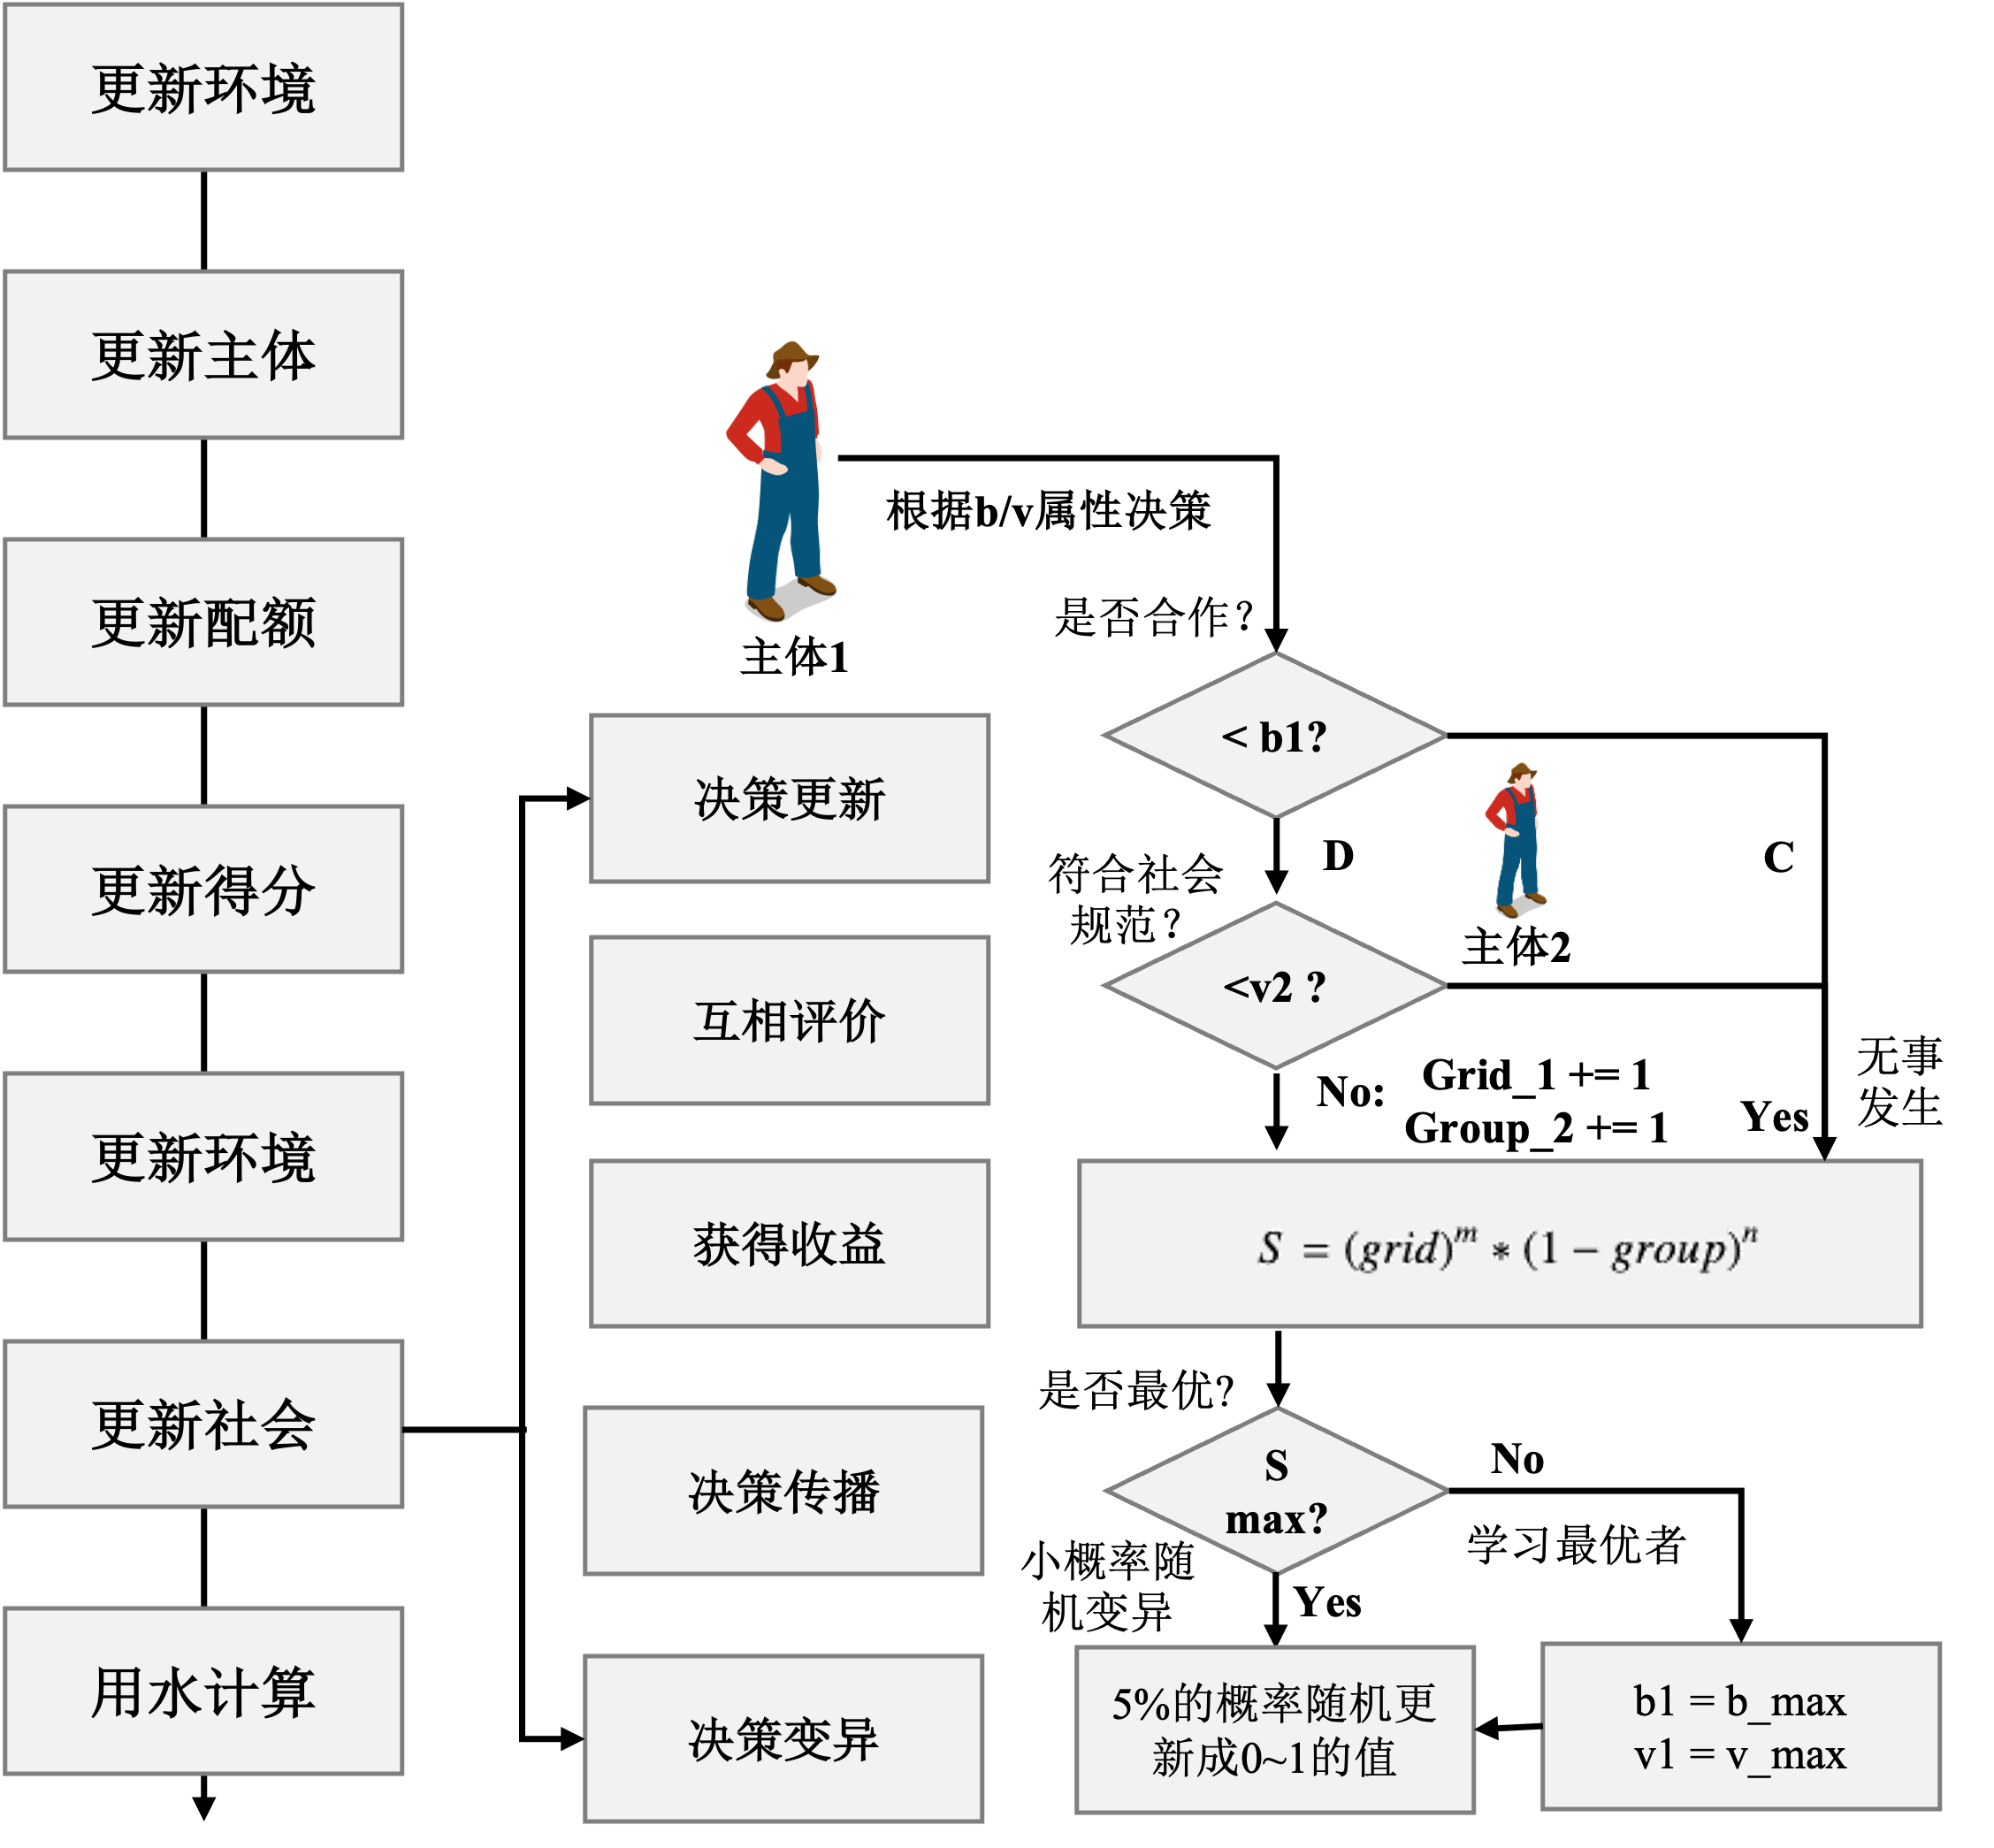
\includegraphics[width=0.8\textwidth]{img/ch6/ch6_updates_diagram.png}
    \caption[多主体模型的更新规则与模拟流程]{多主体模型的更新规则与模拟流程。
    左侧表示多主体模型整体运行的大致流程,“更新社会”步骤是人类模块进行决策的部分,包括五个主要步骤:
        (1)主体根据自己当前的$b$属性(“注重/轻视规范”)作为选择合作的概率,决定本轮中使用的决策“C/D”。
        (2)若当前主体选择不合作(D),其余选择合作(C)的主体根据其$v$属性(“个体/集体主义”)决定是否对其进行社会规范上的谴责。
        (3)对每个主体按照谴责他人/被他人谴责的次数估计自己的社会收益$S$。
        (4)综合社会收益$S$和经济收益$E$,每个主体都将学习自己朋友中综合表现最好的个体,模仿他的$v$和$b$属性,若自己的表现就是朋友中最好的,则跳过此步骤。
        (5)为避免模型陷入局部最优,以极小概率($\alpha = 5\%$)对主体的策略进行变异,设置$v, b \in [0, 1]$成新的随机数。
    }\label{ch6:fig:society}
\end{figure}

\subsubsection{自然模块}

在自然模块中,本研究使用 FAO56 推荐的算法计算潜在蒸散发$ET_0$、作物蒸散系数$Kc$、以及作物蒸散发$ET_c$:

\begin{equation}
    ET_c = ET_0 * Kc * Ks
    \label{ch6:eq:etc}
\end{equation}

其中$Ks$是水应力系数,主要与土壤质地有关。由于在本研究中仅考虑三种主要粮食作物,且主要分布在灌溉条件良好的土壤上,对此系数的空间分异不再作进一步考虑,使用系数$Ks = 0.3$进行估计,作物蒸散发系数$Kc$的同样通过查阅采用国际粮农组织(FAO56)推荐的作物表得到(表\ref{ch6:tab:crops})\cite{chen2023},潜在蒸散发$ET_0$的计算方法使用Penman-Monteith方法,式\ref{ch6:eq:pm}:

\begin{equation}
    \label{ch6:eq:pm}
    PET = \frac{0.408 \Delta (R_{n}-G)+\gamma \frac{900}{T+273}
    (e_s-e_a) u_2}{\Delta+\gamma(1+0.34 u_2)}
\end{equation}

其中$Rn$为作物表面上的净辐射,$MJ/(m^2 day)$;$G$为土壤热通量,$MJ/(m^2 day)$;$T$为$2$米高处日平均气温$^\circ C$;$u_2$为$2$米高处的风速,$m/s$;$es$为饱合水汽压,$kPa$;$ea$为实际水汽压$kPa$;$es - ea$为饱和水汽压差,$kPa$;为饱和水汽压曲线的斜率;$r$为湿度计常数,$kPa/^\circ C$。
由于计算的时间精度为逐月,土壤热通量可以忽略。根据其它数据可得性,对经验公式\ref{ch6:eq:pm}中的饱和水汽压$es$使用气温数据进行估算:

\begin{equation}
    e^0(T) = 0.6108 * \exp \frac{17.27 T}{T + 237.3}
\end{equation}

\begin{equation}
    es = \frac{e^0(T_{\max}) + e^0(T_{\min})}{2}
\end{equation}

作物生长期间的作物系数$Kc$的曲线是用三个阶段的作物系数来估计的:初期($Kc_{ini}$)、中期($Kc_{mid}$)和后期($Kc_{end}$)。
作物系数的各转折点以表\ref{ch6:tab:crops}中的数据为依据进行定位。
$Kc_{ini}$的计算方法如下\cite{allen1998}。

\begin{equation}
    \label{ch6:eq:kcini}
    K_{\text {c, ini}}=\frac{\mathrm{TEW}-(\mathrm{TEW}-\mathrm{REW}) \exp \left[-\left(\mathrm{t}_w-\mathrm{t}_1\right) E_{so}\left(1+\frac{\mathrm{REW}}{\mathrm{TEW}-\mathrm{REW}}\right)\right]}{\mathrm{t}_w E T_{\mathrm{o}}}
\end{equation}

其中,$TEW$为总的可蒸发水量($mm$);$REW$为易蒸发水量($mm$);$tw$为初始时期湿润事件之间的平均时间(天);$t_1$为易蒸发水量干燥完成所需的时间(天);$Eso$为由于低含水层湿润土壤或由于以前干燥时期储存在表层的热量而增加的蒸发潜力($mm/d$)。其中$E_{so} = 1.15 * ET_0$, $t_w = \frac{L_{ini}}{n_w + 0.5}$, $t_1 = REW / E_{so}$。

当$t_1 < t_w$的时候,$K_{\text {c, ini}} = 1.15$,否则使用\ref{ch6:eq:kcini}进行估计,且用来$TEW_{cor}$和$REW_{cor}$替代$TEW$和$REW$。

对于渗透深度$depth < 10mm$的所有土壤质地,有:

\begin{equation}
    TEW_{cor} = 10mm \\
    REW_{cor} = \min(\max(2.5, 6 / ET_0^{0.5}, 7))
\end{equation}

对于渗透深度$depth \geqq 40mm$的所有土壤质地,有:

\begin{equation}
    TEW_{cor} = \min(15, 7 {(ET_0)}^{0.5}) \\
    REW_{cor} = \min(6, TEW_{cor} - 0.01)
\end{equation}

适用于渗透深度$depth \geqq 40mm$的中、细土质,有:

\begin{equation}
    TEW_{cor} = \min(28, 13{(ET_0)}^{0.5}) \\
    REW_{cor} = \min(9, TEW_{cor} - 0.01)
\end{equation}

对于$depth \in (10mm, 40mm)$,有:
\begin{equation}
    K_{c, ini} = K_{c, ini(I \leqq 10mm)} + \frac{I-10}{40-10}[K_{c, ini(I>10mm)} - K_{c, ini(I \leqq 10mm)}]
\end{equation}

其中,$K_{c, ini(I \leqq 10mm)}$是指入渗深度 $depth \leqq 10 mm$的所有土壤质地的$K_{c, ini}$值;$K_{c, ini(I > 40 mm)}$是指入渗深度$depth>40 mm$的粗或中/细土壤质地的$K_{c, ini}$值。

$K_{c, mid}$ 可以由下式估计:
\begin{equation}
    K_{c, mid} = K_{c, mid(Tab)} + [0.04(u_2 - 2) -0.004(RH_{\min} - 45)]{(\frac{h}{3})}^{0.3}
\end{equation}

$K_{c, end}$ 可以由下式估计:
\begin{equation}
    K_{c, end} = K_{c, end(Tab)} + [0.04(u_2 - 2) -0.004(RH_{\min} - 45)]{(\frac{h}{3})}^{0.3}
\end{equation}

其中 $K_{c, mid(Tab)}$ 和 $K_{c, end(Tab)}$ 均是 FAO 作物表中推荐的估计值(见表\ref{ch6:tab:crops})。
完成各阶段作物系数计算后,参考作物的生长周期还原当年的作物系数曲线,并通过按月平均匹配本研究的尺度。

\subsubsection{人地模块的耦合}

本章研究的模型在基于地理数据的多主体建模框架“ABSESpy”基础上搭建,这是一个多主体建模开源框架软件包\cite{song2023}。
该框架使用真实的地理空间数据集来构建人工社会生态系统,同时充分考虑人类行为因素。
它支持使用地理空间数据,对具有认知、社会影响和反应等行为的主体进行建模,用户可以专注于分别实现人类行为的逻辑和自然过程的仿真,该框架使得两者之间能够轻松地访问和修改变量值,该框架可以调度任意数量的自然模块和社会模块,并使它们之间松散耦合。

在本章研究中,人类用水模块通过作物种植来改变自然模块的作物地表覆被属性,自然模块则通过降水、地表蒸散发的变化来影响人类用水模块中的决策环境,主体可以根据其所在位置调用相关的自然属性,所有主体、环境间相互感知能力如表\ref{ch6:tab:visa3}所示,主体的所有模型行为总结在表\ref{ch6:tab:visa4}中。

% % Table generated by Excel2LaTeX from sheet '主体属性描述'
% % \begin{landscape}
% \begin{sidewaystable}[htbp]
%     \centering
%     \caption{多主体模型主体属性描述}
%     \begin{tabularx}{\textheight}{LLLLL p{5cm}}
%       \toprule
%       \multicolumn{1}{l}{主体实例} & 符号    & 内生/外生 & 数据类型  & 单位    & 说明 \\
%       \midrule
%       \multicolumn{1}{l}{e1: 栅格} & $pop_{x, y}$ & 外生    & 整型    & 人     & 人口分布 \\
%             & $ETc_{x, y}$ & 内生    & 浮点数   & 毫米    & 作物蒸散发 \\
%             & $Kc_{x, y}$ & 内生    & 浮点数   & 无量纲   & 作物蒸散发系数 \\
%             & $prec_{x, y}$ & 外生    & 浮点数   & 毫米    & 降水量 \\
%       \multicolumn{1}{l}{e2: 社会网} & $nf_{hub, c1}$ & 外生    & 整型    & 个     & 各地级市可与其它市农民产生社会联系的关键农民数量 \\
%             & $p_n$ & 外生    & 浮点数   & 无量纲   & 各地级市内农民主体之间产生社会联系的概率 \\
%             & $p_C$ & 外生    & 浮点数   & 无量纲   & 各省关键农民之间产生社会联系的概率 \\
%       \multicolumn{1}{l}{e3: 全局环境} & ${Q_{\max, c1}, Q_{\max, c2} \dots}$ & 外生    & 浮点数   & 立方米   & 各地级市可供地表水的上限 \\
%             & ${Q_{\min, c1}, Q_{\min, c2} \dots}$ & 外生    & 浮点数   & 立方米   & 各地级市当前的官方地表水配额 \\
%             & $Ke$  & 外生    & 浮点数   & 无量纲   & 灌溉损失系数 \\
%             & $res$ & 外生    & 浮点数   & 度     & 分辨率 \\
%             & $Ks$  & 外生    & 浮点数   & 无量纲   & 水应力系数 \\
%             & $grid$ & 外生    & 浮点数   & 无量纲   & 社会规范中违规意愿的水平 \\
%             & $group$ & 外生    & 浮点数   & 无量纲   & 社会规范中从中意愿的水平 \\
%       \multicolumn{1}{l}{农民} & $crop$ & 外生    & 字符串   & 无     & 作物类型(玉米/小麦/水稻) \\
%             & $neighbors$ & 外生    & 农民集合  & 无     & 与自己存在社会联系的农民主体集合 \\
%             & $province$ & 外生    & 字符串   & 无     & 所在省份(依据GIS数据) \\
%             & $city$ & 外生    & 字符串   & 无     & 所在地级市(依据GIS数据) \\
%             & $wui$ & 外生    & 浮点数   & 毫米    & 当年的灌溉用水效率 \\
%             & $mut$ & 外生    & 浮点数   & 浮点数   & 个体属性随机变异的概率 \\
%             & $q_{\min}$ & 内生    & 浮点数   & 毫米    & 能分配给当前农民的最小地表水额度 \\
%             & $q_{\max}$ & 内生    & 浮点数   & 毫米    & 能分配给当前农民的最大地表水额度 \\
%             & $b$   & 内生    & 浮点数   & 无量纲   & 违规意愿 \\
%             & $v$   & 内生    & 浮点数   & 无量纲   & 从众意愿 \\
%             & $d$   & 内生    & 字符串   & 无     & 分类(合作/不合作) \\
%             & $s$   & 内生    & 浮点数   & 无量纲   & 社会得分 \\
%             & $e$   & 内生    & 浮点数   & 无量纲   & 经济得分 \\
%             & $u$   & 内生    & 浮点数   & 无量纲   & 总得分 \\
%             & $demands$ & 内生    & 浮点数   & 毫米    & 当月的用水需求 \\
%             & $deficits$ & 内生    & 浮点数   & 毫米    & 当月的灌溉水亏缺 \\
%             & $quota$ & 内生    & 浮点数   & 毫米    & 当月实际地表用水配额 \\
%             & $m$   & 内生    & 整型    & 次     & 发现朋友违规的次数 \\
%             & $n$   & 内生    & 整型    & 次     & 被朋友发现违规的次数 \\
%             & $gw$  & 内生    & 浮点数   & 毫米    & 当月地下水使用量 \\
%             & $gs$  & 内生    & 浮点数   & 毫米    & 当月地表水使用量 \\
%         \bottomrule
%       \end{tabularx}%
%     \label{ch6:tab:visa2}%
%   \end{sidewaystable}%
% % \end{landscape}


% Table generated by Excel2LaTeX from sheet '主体属性描述'
\begin{table}[htbp]
      \centering
      \caption{多主体模型环境属性描述}
        \begin{tabularx}{\textwidth}{LLLLp{6cm}}
        \toprule
        符号    & 内生/外生 & 数据类型  & 单位    & 说明 \\
        \midrule
        $pop_{x, y}$ & 外生    & 整型    & 人     & 人口分布 \\
        $ETc_{x, y}$ & 内生    & 浮点数   & 毫米    & 作物蒸散发 \\
        $Kc_{x, y}$ & 内生    & 浮点数   & 无量纲   & 作物蒸散发系数 \\
        $prec_{x, y}$ & 外生    & 浮点数   & 毫米    & 降水量 \\
        $nf_{hub, c}$ & 外生    & 整型    & 个     & 地级市$c$可与其它市农民产生社会联系的关键农民数量 \\
        $p_n$ & 外生    & 浮点数   & 无量纲   & 各地级市内农民主体之间产生社会联系的概率 \\
        $p_C$ & 外生    & 浮点数   & 无量纲   & 各省关键农民之间产生社会联系的概率 \\
        ${Q_{\max, c}}$ & 外生    & 浮点数   & 立方米   & 地级市$c$可供地表水的上限 \\
        ${Q_{\min, c}}$ & 外生    & 浮点数   & 立方米   & 地级市$c$当前的官方地表水配额 \\
        $k_{loss}$  & 外生    & 浮点数   & 无量纲   & 灌溉损失系数 \\
        $res$ & 外生    & 浮点数   & 度     & 分辨率 \\
        $Ks$  & 外生    & 浮点数   & 无量纲   & 水应力系数 \\
        $grid$ & 外生    & 浮点数   & 无量纲   & 社会规范中违规意愿的水平 \\
        $group$ & 外生    & 浮点数   & 无量纲   & 社会规范中从中意愿的水平 \\    
        \bottomrule
        \end{tabularx}%
      \label{ch6:tab:visa2.env}%
\end{table}%


% Table generated by Excel2LaTeX from sheet '主体属性描述'
\begin{table}[htbp]
      \centering
      \caption{多主体模型人类模块的属性描述}
        \begin{tabularx}{\textwidth}{LLLLp{6cm}}
        \toprule
        符号    & 内生/外生 & 数据类型  & 单位    & 说明 \\
        \midrule
        $crop$ & 外生    & 字符串   & 无     & 作物类型(玉米/小麦/水稻) \\
        $neighbors$ & 外生    & 农民集合  & 无     & 与自己存在社会联系的农民主体集合 \\
        $province$ & 外生    & 字符串   & 无     & 所在省份(依据GIS数据) \\
        $city$ & 外生    & 字符串   & 无     & 所在地级市(依据GIS数据) \\
        $wui$ & 外生    & 浮点数   & 毫米    & 当年的灌溉用水效率 \\
        $mut$ & 外生    & 浮点数   & 浮点数   & 个体属性随机变异的概率 \\
        $q_{\min}$ & 内生    & 浮点数   & 毫米    & 能分配给当前农民的最小地表水额度 \\
        $q_{\max}$ & 内生    & 浮点数   & 毫米    & 能分配给当前农民的最大地表水额度 \\
        $b$   & 内生    & 浮点数   & 无量纲   & 违规意愿 \\
        $v$   & 内生    & 浮点数   & 无量纲   & 从众意愿 \\
        $d$   & 内生    & 字符串   & 无     & 分类(合作/不合作) \\
        $s$   & 内生    & 浮点数   & 无量纲   & 社会得分 \\
        $e$   & 内生    & 浮点数   & 无量纲   & 经济得分 \\
        $u$   & 内生    & 浮点数   & 无量纲   & 总得分 \\
        $demands$ & 内生    & 浮点数   & 毫米    & 当月的用水需求 \\
        $deficits$ & 内生    & 浮点数   & 毫米    & 当月的灌溉水亏缺 \\
        $quota$ & 内生    & 浮点数   & 毫米    & 当月实际地表用水配额 \\
        $m$   & 内生    & 整型    & 次     & 发现朋友违规的次数 \\
        $n$   & 内生    & 整型    & 次     & 被朋友发现违规的次数 \\
        $gw$  & 内生    & 浮点数   & 毫米    & 当月地下水使用量 \\
        $gs$  & 内生    & 浮点数   & 毫米    & 当月地表水使用量 \\
        \bottomrule
        \end{tabularx}%
      \label{ch6:tab:visa2.hum}%
    \end{table}%
    

% Table generated by Excel2LaTeX from sheet '主体感知'
\begin{table}[htbp]
    \centering
    \caption{多主体模型中主体与环境的感知情况}
      \begin{tabularx}{0.6\textwidth}{LLL}
      \toprule
            & 环境    & 农民 \\
      \midrule
      环境    & $*$     & \{$f_{crop} \dots$\} \\
      农民    & $prec$, $ET_c$ & $[*] d, p, b, v$ \\
      \bottomrule
      \end{tabularx}%
    \label{ch6:tab:visa3}%
\end{table}%

% Table generated by Excel2LaTeX from sheet '行为描述'
% \begin{landscape}
  \begin{sidewaystable}[htbp]
    \centering
    \caption{多主体模型的主体行为描述}
      \begin{tabularx}{\textheight}{LLLLLLLLL}
      \toprule
      \multicolumn{1}{l}{主体} & 行为名称  & 感知自身属性 & 感知其它主体属性 & \multicolumn{1}{l}{行为模型} & 被改变的自身属性 & \multicolumn{1}{l}{被改变的其它主体属性} & 执行条件  & 相关公式 \\
      \midrule
      \multicolumn{1}{l}{环境E} & 添加/移除农民 & $pop_{x, y}$ &       & \multicolumn{1}{l}{加权平均} & $n_f$ &       & 每年    & 无 \\
            & 计算作物蒸散发 & $ET_0$ & ${f_{crop} \dots}$ & \multicolumn{1}{l}{自然过程} & $ET_c, Kc_{ini}, Kc_{mid}, Kc_{end}$ &       & 每月    & 式\ref{ch6:eq:etc} \\
      \multicolumn{1}{l}{农民f} & 决定用水来源 & $quota, demands$ & $prec, etc$ & \multicolumn{1}{l}{if-else rules} & $gw, sw$ &       & 每月    & 式\ref{ch6:eq:wu} \\
            & 做出超采决定 & $b, demands$ & $prec$ & \multicolumn{1}{l}{if-else rules} & $quota$ &       & 每月    & 式\ref{ch6:eq:quota} \\
            & 从表现好的朋友处学习 & $neighbors, u, b, v, p_{mut}$ & $u, b, v$ & \multicolumn{1}{l}{if-else rules} & $b, v$ &       & 每年    & 无 \\
            & 监督朋友违规情况 & $neighbors, v$ & $d$   & \multicolumn{1}{l}{if-else rules} & $m$   & \multicolumn{1}{l}{$n$} & 每年    & 无 \\
            & 计算得分  & $gw, m, n$ & $grid, group$ &       & $m, n, e, s$ &       & 每年    & 式\ref{ch6:eq:society}、式\ref{ch6:eq:score} \\  
      \bottomrule
      \end{tabularx}%
    \label{ch6:tab:visa4}%
  \end{sidewaystable}%
% \end{landscape}
\subsection{数据处理}

\subsubsection{输入数据}

本章研究使用的数据清单如表\ref{ch6:tab:dataset}所示,包括气象数据、作物物候数据、灌溉面积和灌溉用水数据、用水配额数据、人口数据等,其中较为重要且需要预处理的主要是来自黄河水利委员会公开的水资源配额数据。
该数据仅在2014年后才公开了逐月精度的数据,但包括了每个月水量相较于多年平均水平相差的百分比(即表\ref{ch6:tab:dataset}中所示的距平)。
因此,本研究首先根据该距平值将逐月的配额推演至多年平均水平,进一步假设该水量分配是按各地区实际需求分配的,利用用水量数据将省尺度的配额降尺度到地级市。
例如,对某个属于$I$省的地级市$i$在月份$j$内的灌溉用水配额$Q_{ij}$估计为:

\begin{equation}
    \label{ch6:eq:quota_data}
    Q_{ij} = Q_{I, j} * \frac{WU_{i, j}}{\sum_{j = 1, 2, \dots, 12} WU_{I}}
\end{equation}

由于此分水水量包括了所有产业、所有类型灌溉耕地,所以通过式\ref{ch6:eq:quota_data}计算所得该分水额度$Q$需要进行进一步按比例作细化处理:

\begin{equation}
    Q_{W, R, M} = W_{W, R, M} / WU_{sum} * Q
\end{equation}

其中$W, R, M$分别是本研究主要关注的小麦、水稻、玉米三种黄河流域主要作物的用水量,$WU_{sum}$为该地区的总用水量,利用两者的比例作为系数对此地区的用水额度作进一步按需分配,作为本研究多主体模型中研究三种作物所使用的额度数据。

% Table generated by Excel2LaTeX from sheet '数据来源表'
\begin{table}[htbp]
    \centering
    \caption{多主体模型的数据源}
      \begin{tabularx}{\textwidth}{LLLLLL}
      \toprule
      数据名称  & 变量    & 使用数据的模块 & 模型使用描述 & 时间精度  & 数据来源 \\
      \midrule
      中国区域地面气象要素驱动数据集 & 气温、风速、气压、降水、辐射 & 自然模块  & 计算潜在蒸散发 & 1979年至今,0.1度分辨率,逐月 & 中国区域地面气象要素驱动数据集 \\
      作物物候数据 & 物候生长期 & 自然模块  & 计算作物蒸散发 & 全中国干旱/半干旱区 & 文献(已接收) \\
      灌溉配额数据 & 灌溉配额及其距平 & 人类模块  & 估算用水配额 & 2014年迄今,逐月 & 黄河水利委员会网站 \\
      黄河流域用水数据 & 灌溉面积、灌溉用水量 & 模型规则  & 估算主体数量 & 1965年至2013年逐年 & 文献\cite{zhou2020} \\
      人口分布数据 & 人口数量  & 模型规则  & 生成主体分布位置的概率 & 仅2010年一期 & WorldPop\cite{worldpop2020} \\
      \bottomrule
      \end{tabularx}%
    \label{ch6:tab:dataset}%
  \end{table}%
  

\subsubsection{参数选取}

本研究所有的参数(见表\ref{ch6:tab:visa2.env}、表\ref{ch6:tab:visa2.hum})估计都有前人研究作为参考,需要特别说明的参数选取及其意义主要有三部分:
(1)影响人类模块得分计算的两个社会效用函数在过往的研究中已经被多次使用,且基于问卷数据进行了较为可靠的估计,本研究直接参考Castilla-Rho 研究中从世界价值观调查数据库中对这两个参数的估计值\cite{castilla-rho2015, castilla-rho2017, castilla-rho2020}。
(2)自然模块的$Ks$是水应力系数,主要与土壤质地有关。由于在本研究中仅考虑三种主要粮食作物,且主要分布在灌溉条件良好的土壤上,对此系数的空间分异不再作进一步考虑,使用系数$Ks = 0.3$进行估计。灌溉损失系数则是经验值$0.8$,代表无论如何都有$20\%$的水分会在灌溉中损失掉。
(3)人类模块的$p_l$概率、模型规则中的$p_n$、$p_C$参数都与社会网络的形成有关。
Francisco 等人的研究已经对网络结构对演化博弈决策行为传播的影响做了很经典的研究\cite{santos2008},本研究将三个概率参数均设置为$1$,即每个省区都将形成典型的“星形网络”,根据其研究结果,这是一种促进决策传播的有效结构,广泛存在且与已有文献之间具备可对比性\cite{santos2008}。
此外,根据罗家德等人的研究,这也较为符合我国地方社会“以能人为核心”的关系网络结构\cite{luojiade2013}。

\subsubsection{分析方法和工具}

本研究使用广义加性模型(Generalized Additive Models, GAM)分析地区用水量随时间变化的趋势,这是一种广泛应用于回归分析的非参数统计模型。
相比于线性回归模型,GAM 没有对因变量和自变量之间的关系做出先验假设,因此在数据非线性、非正态分布、存在交互作用等情况下更具有优势。
GAM 通过使用光滑的非参数函数(如样条函数)对自变量的影响进行建模,同时也可以应用广义线性模型中的方法来对非正态数据进行回归分析。

所有模型使用Python软件3.11版本进行构建,使用到的软件包均为开源软件,版本及其用途如表\ref{ch6:tab:packages}所示。
% 本章构建的多主体模型暂时不予以开源,但具体构建方式已在上述方法中进行了详尽描述。

% Table generated by Excel2LaTeX from sheet '使用包一览表'
\begin{table}[htbp]
    \centering
    \caption{多主体模型使用的开源软件包}
      \begin{tabularx}{0.9\textwidth}{p{2cm} p{1.5cm} L}
        \toprule
      名称    & 版本号   & 描述 \\
      \midrule
      ABSESpy & 0.1.3 & 自动建设简单的 ABM 模型 \\
      hydra-core & 1.3.2 & 简化应用程序的配置 \\
      xarray & 2023.2.0 & 处理标记数据数组的 Python 库 \\
      rasterio & 1.3.6 & 用于读写栅格数据的 Python 库 \\
      geopandas & 0.12.2 & 处理地理空间数据的 Python 库 \\
      rioxarray & 0.13.4 & Rasterio + xarray:利用 xarray 的能力读取和处理栅格数据 \\
      networkx & 3.0 & 创建、操作和学习复杂网络的工具 \\
      dataclasses-json & 0.5.7 & 将数据类编码为 JSON 的 Python 库 \\
      China-Water-Uses & 0.1.0 & 加载、组织和绘制中国用水数据 \\
      fiona & 1.9.1 & 读写 GIS 数据格式的 Python 库 \\
      seaborn & 0.12.2 & 用于绘制漂亮且有信息量的统计图形的 Python 库 \\
      geocube & 0.4.0 & 将栅格数据转换为向量数据的 Python 库 \\
      pygam & 0.8.0 & Python 的 GAM 工具 \\
      \bottomrule
      \end{tabularx}%
    \label{ch6:tab:packages}%
  \end{table}%
  
